\chapter{Návrh testov pre systém Fitcrack}
K~návrhu testov pre systém Fitcrack potrebujeme poznať:
\begin{itemize}
	\item architektúru systému Fitcrack~\ref{Fitcrack},
	\item moduly, ktoré budú testované~\ref{tests_moduls},
	\item kedy budú ktoré moduly testované~\ref{test_design},
	\item spôsoby testovania~\ref{testing_levels},
\end{itemize}
Fitcrack pozostáva z niekoľkých častí, tak ako sú navrhnuté v systéme BOINC~\cite{boincintro}.
V mojej práci som sa rozhodol testovať s použitím zdrojových kódov, kedže nemám k dispozícii kompletnú špecifikáciu systému, alebo jeho komponentov. 
Tvorba testov vychádza z požiadaviek na konkrétny komponent.
U modulu generátor a asimilátor, ktorých činnosť je popísaná pseudokódom~\ref{alg:generator} a~\ref{alg:asimilator} som sa rozhodol vytvoritť CFG a vytvoriť požiadavky na základe prechodu grafu. 
Na nájdenie primárnych ciest grafu som použil nástroj Prime Path Coverage\footnote{\url{https://github.com/heshenghuan/Prime-Path-Coverage}}.

Podľa Google blog o testovaní\footnote{\url{http://blog.codepipes.com/testing/software-testing-antipatterns.html}} spadajú do kategórie integračných testov~\ref{integration_tests}, no každý test testuje iba jediný modul, takže budem používať názov testovanie modulov.

\section{Návrh testov pre modul generátor}
Generátor má na starosti generovanie nových úloh pre klientov a rozdeľovanie nových, či neúspešne dokončených úloh. 
Komunikuje výhradne s databázou, beží v nekonečnom cykle, kde periodicky kontroluje bežiace balíky a ak je to potrebné generuje nové úlohy, alebo prerozdeľuje neúspešne dokončené úlohy.

Pre testovanie bol pôvodný zámer implementovať pokrytie primárny ciest~\ref{kriteria_cfg}, no po vygenerovaní všetkých primárnych ciest pomocou vyššie spomínaného program Prime path coverage bolo od tohto zámeru upustené, hlavne kvôli rozsahu, kedže počet primárnych ciest bol 777.
Nakoniec som uznal za vhodné vybrať kritérium pokrytia všetkých uzlov (node coverage).


\begin{figure}[h]
	\centering
	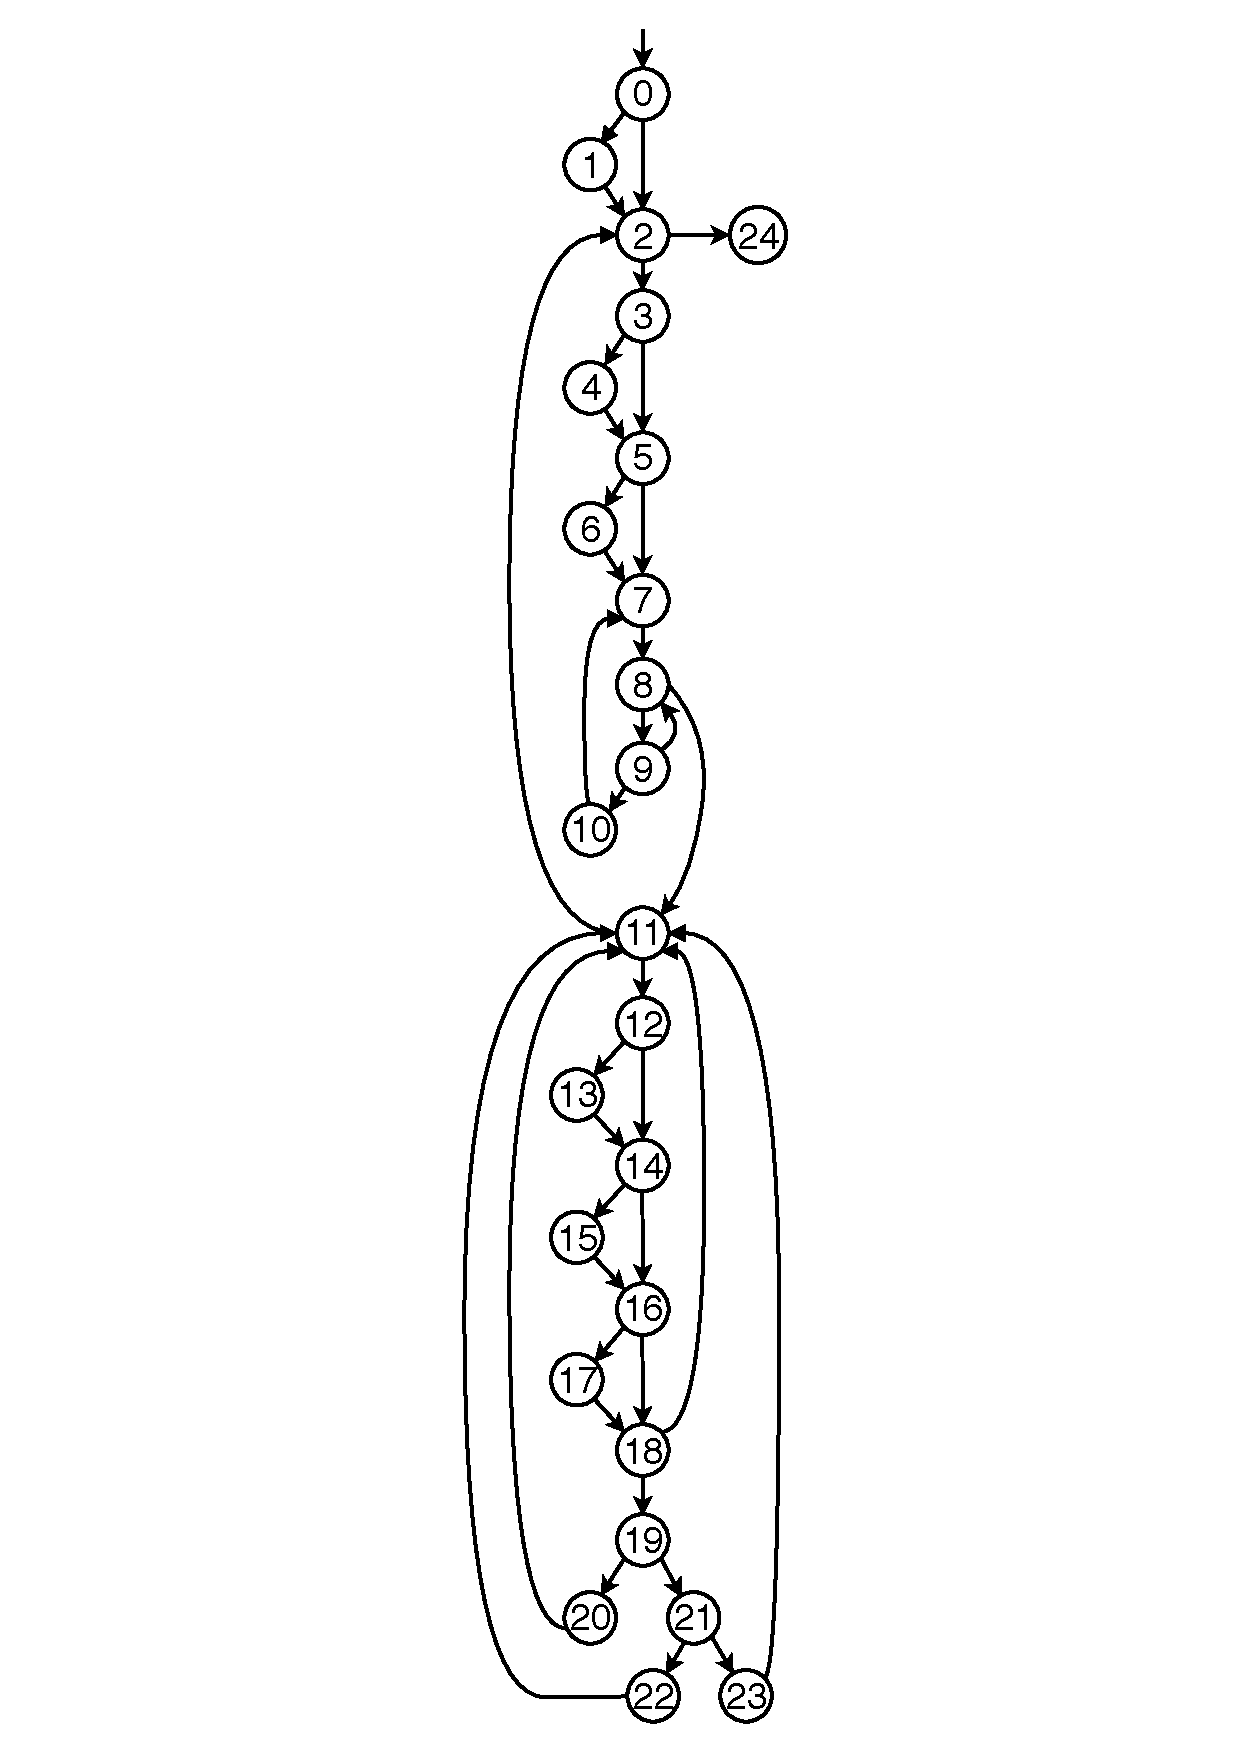
\includegraphics[height=0.7\paperheight]{obrazky/cfg_generator.pdf}
	\caption{CFG generátora~\ref{alg:generator}.}
	\label{fig:cfg_gen}
\end{figure}

\section{Návrh testov pre modul asimilitátor}

\begin{figure}[h]
	\centering
	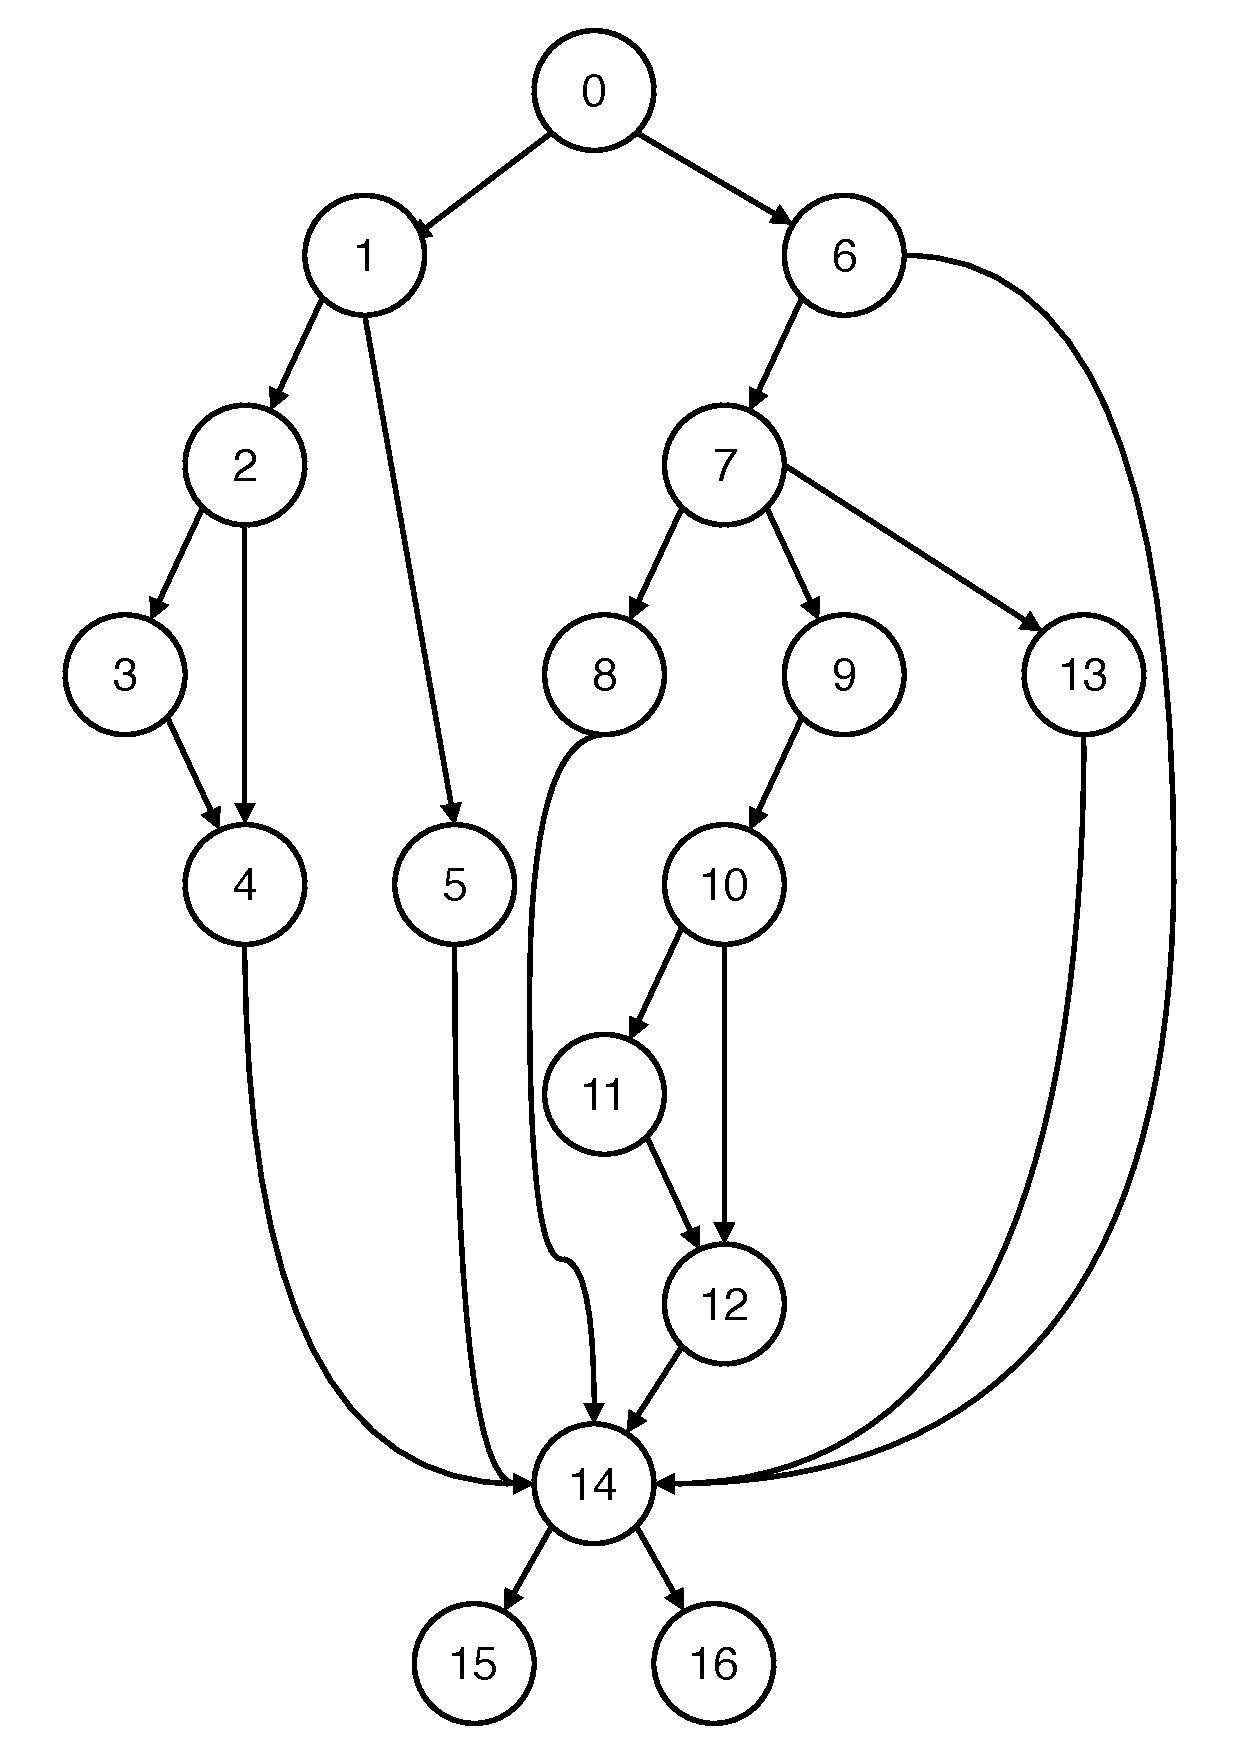
\includegraphics[height=0.7\paperheight]{obrazky/cfg_asimilator.pdf}
	\caption{CFG asimilátora~\ref{alg:asimilator}.}
	\label{fig:cfg_asim}
\end{figure}
\section{Návrh testov pre modul runner}

\section{Návrh testov pre API}

\chapter{Implementácia}
\section{Použité technológie}
\section{Implementácia testov pre serverový modul assimilátor}
\section{Implementácia testov pre serverový modul generátor}
\section{Implementácia testov pre modul runner}
\section{Implementácia testov aplikačného rozhrania }
